% Template for ICIP-2013 paper; to be used with:
%          spconf.sty  - ICASSP/ICIP LaTeX style file, and
%          IEEEbib.bst - IEEE bibliography style file.
% --------------------------------------------------------------------------
\documentclass{article}
\usepackage{spconf,amsmath,graphicx, subfigure}

% Example definitions.
% --------------------
\def\x{{\mathbf x}}
\def\L{{\cal L}}

% Title.
% ------
\title{Advantages of Subspace Estimation Techniques over Gaussian Mixture Models for Background Subtraction of Noisy Videos}
%
% Single address.
% ---------------
\name{Pooya Khorrami, Xingqian Xu, Mert Dikmen, Thomas S. Huang\thanks{Thanks to XYZ agency for funding.}}
\address{University of Illinois - Urbana Champaign \\ 
              Department of Electrical and Computer Engineering\\
              Beckman Institute,  405 N. Matthews Avenue, Urbana IL, 61801}
%
% For example:
% ------------
%\address{School\\
%	Department\\
%	Address}
%
% Two addresses (uncomment and modify for two-address case).
% ----------------------------------------------------------
%\twoauthors
%  {A. Author-one, B. Author-two\sthanks{Thanks to XYZ agency for funding.}}
%	{School A-B\\
%	Department A-B\\
%	Address A-B}
%  {C. Author-three, D. Author-four\sthanks{The fourth author performed the work
%	while at ...}}
%	{School C-D\\
%	Department C-D\\
%	Address C-D}
%
\begin{document}
%\ninept
%
\maketitle
%
\begin{abstract}
The abstract should appear at the top of the left-hand column of text, about
0.5 inch (12 mm) below the title area and no more than 3.125 inches (80 mm) in
length.  Leave a 0.5 inch (12 mm) space between the end of the abstract and the
beginning of the main text.  The abstract should contain about 100 to 150
words, and should be identical to the abstract text submitted electronically
along with the paper cover sheet.  All manuscripts must be in English, printed
in black ink.
\end{abstract}
%
\begin{keywords}
One, two, three, four, five
\end{keywords}
%

%\vspace{0.5in}

\section{Introduction}
%\label{sec:intro}
In the field of video surveillance, the user typically wishes to extract meaningful and salient information from a video sequence in a completely automatic fashion. In several instances, the video sequences are captured using stationary cameras leading to a relatively static scene layout. The absence of camera motion implies that the background of the video sequence exhibits very little variation while dynamic changes in the scene represent the objects of interest. In such a case, the most common approach is to perform background subtraction to separate said dynamic regions (i.e. foreground) from the background of each frame.

When performing background subtraction, some na\"ive methods include frame differencing and approximate median \cite{approxMed}. %Frame difference simply subtracts the current frame from the previous frame and the pixels where the difference exceeds a threshold are marked as foreground. The approximate median technique, on the other hand, models the background as the median of several past frames in the sequence. This median image is then subtracted from subsequent frames and pixels whose difference exceed a threshold are marked foreground. 
While these algorithms are simple to use and quite efficient, the most popular technique, by far, is adaptive  Gaussian Mixture Models (GMMs) \cite{FriedmanGMM, StaufferGMM}. These works posit that each pixel in the background image can be represented by a probability distribution formed by a mixture of Gaussians. If a pixel greatly deviates from its corresponding model, then the pixel is labeled foreground. While the number of Gaussians used at each pixel is usually fixed, there has been some work \cite{ZivGMM} that adaptively selects the number of mixture components.

Although background subtraction via Gaussian Mixture Models enjoys widespread use in the computer vision community, it is not without drawbacks. As opposed to the frame differencing and approximate median techniques, GMMs possess several parameters that must be individually tuned. This implies that the algorithm is innately sensitive to different scene configurations. Therefore it should be no surprise that GMMs tend to perform rather poorly on noisy videos where the foreground objects are not immediately distinguishable. 

When dealing with noisy video sequences, we advocate the use of low-rank subspaces for background subtraction.  Given that each of the video sequences was obtained using a stationary camera, the high level of temporal redundancy between the frames suggests that the backgrounds lie on a low-dimensional subspace. Therefore, foreground activity can be thought of as sparse deviations from said subspace. In this paper, we consider two different subspace estimation algorithms and show empirically how they both achieve superior performance to GMMs on noisy traffic video sequences. 

The first method,  Robust Principal Component Analysis (RPCA or Robust PCA) \cite{RPCA09}, attempts to decompose a data matrix (or video sequence) into a low-rank matrix and a sparse matrix via a convex optimization problem. While typically performed in batch on purely intensity videos, we describe how performing Robust PCA on each of the color channels of video and subsequent post processing via wavelet de-noising leads to additional performance gains. If a user requires a real-time alternative, we also consider the newly proposed Grassmannian Robust Adaptive Subspace Tracking Algorithm (GRASTA) by He et al. \cite{GRASTA12} that learns the aforementioned low-rank subspace by subsampling the video frames and proceeds in an online fashion. 

The remainder of this paper is organized as follows. Section 2 will describe the improvements made to the batch Robust PCA algorithm. Section 3 will present our experimental setup and findings. Section 4 will describe our conclusions and directions for future work.


%When dealing with noisy video sequences, we advocate the use of Robust Principal Component Analysis (RPCA or Robust PCA) for background subtraction. Robust PCA \cite{RPCA09} refers to how any matrix M can be represented as the sum of a low-rank matrix L and sparse matrix S by solving a convex optimization problem. If we form the matrix M by stacking each frame of the video sequence as a column, then we will see that the columns are highly correlated. This is expected considering that the video was obtained using a stationary camera and implies that the background of a video scene lies on a low-dimensional subspace. As a result, when Robust PCA is performed on the matrix M, the columns of the low-rank matrix L will correspond to the background of the frame and the columns of the matrix S will contain sparse deviations from the low-rank subspace. 

%While the aforementioned description of Robust PCA operates on a video sequence in batch, there is also the newly proposed Grassmannian Robust Adaptive Subspace Tracking Algorithm (GRASTA) by He et al. \cite{GRASTA12} that learns the low-rank subspace by subsampling the video frames and proceeds in an online fashion. Although it is not Robust PCA in its purest sense, GRASTA still assumes that each frame can be represented as the sum of data generated from a low-dimensional subspace and a sparse error term.

%In this paper, we will show how Robust PCA achieves superior performance to GMMs when applied to noisy videos. We will also describe how performing Robust PCA on each of the color channels of a video sequence and subsequent thresholding of the wavelet coefficients provide additional improvements. Should the user require a real-time alternative, we will also show how GRASTA also outperforms GMMs on the same noisy data. The remainder of this paper is organized as follows. Section 2 will describe the improvements made to the batch Robust PCA algorithm. Section 3 will present our experimental setup and findings. Section 4 will describe our conclusions and directions for future work.

\section{Method Description}
%\label{sec:format}

Traditionally, when given a video sequence, Robust PCA

Up until now, there has been very little work that investigates the gohadigohaoig


\begin{figure*}[htb]

\begin{minipage}[b]{0.3333\linewidth}
  \centering
  \centerline{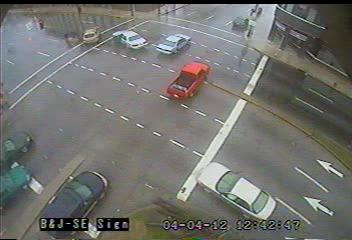
\includegraphics[width=5.55cm]{Imgs/Orig_0412041242.jpg}}
%  \vspace{2.0cm}
  \centerline{(a) Original Image}\medskip
\end{minipage}
%
\begin{minipage}[b]{0.3333\linewidth}
  \centering
  \centerline{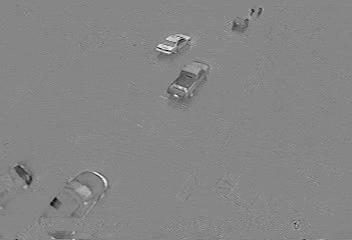
\includegraphics[width=5.55cm]{Imgs/SP_Intensity_0412041242}}
%  \vspace{1.5cm}
  \centerline{(b) Intensity Sparse Image}\medskip
\end{minipage}
\hfill
\begin{minipage}[b]{0.3333\linewidth}
  \centering
  \centerline{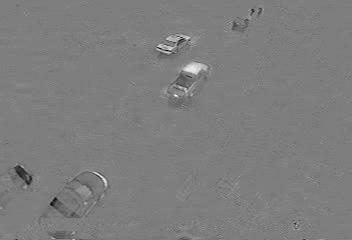
\includegraphics[width=5.55cm]{Imgs/SP_IMG_R_0412041242.jpg}}
%  \vspace{1.5cm}
  \centerline{(c) Red Channel Sparse Image}\medskip
\end{minipage}
%
\caption{Visual Comparison of Robust PCA on Intensity and a Color Channel}
\label{fig:colorComp}
%
\end{figure*}



\begin{figure*}[htb]

\begin{minipage}[b]{0.3333\linewidth}
  \centering
  \centerline{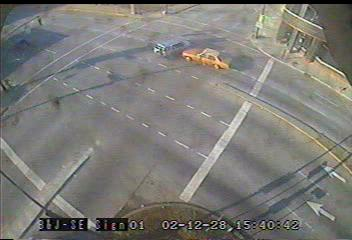
\includegraphics[width=5.55cm]{Imgs/Orig_1228021540.jpg}}
%  \vspace{2.0cm}
  \centerline{(a) Original Image}\medskip
\end{minipage}
%
\begin{minipage}[b]{0.3333\linewidth}
  \centering
  \centerline{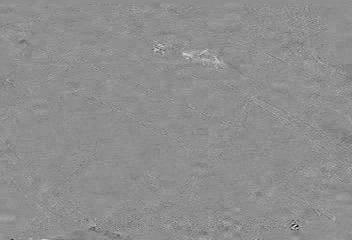
\includegraphics[width=5.55cm]{Imgs/SP_IMG_R_1228021540.jpg}}
%  \vspace{1.5cm}
  \centerline{(b) Robust PCA Sparse Image}\medskip
\end{minipage}
\hfill
\begin{minipage}[b]{0.3333\linewidth}
  \centering
  \centerline{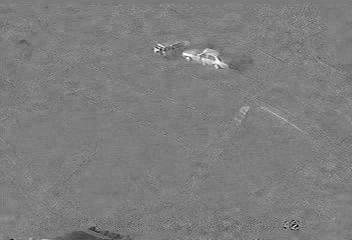
\includegraphics[width=5.55cm]{Imgs/SP_IMG_Reduced_1228021540.jpg}}
%  \vspace{1.5cm}
  \centerline{(c) Reduced Robust PCA Sparse Image}\medskip
\end{minipage}
%
\caption{Reduced Frames Comparison}
\label{fig:interleaveComp}
%
\end{figure*}



\section{Experimental Results}
%\label{sec:pagestyle}

(Cite Toyota Dataset?)

\section{Conclusions}
%\label{sec:typestyle}



% References should be produced using the bibtex program from suitable
% BiBTeX files (here: strings, refs, manuals). The IEEEbib.bst bibliography
% style file from IEEE produces unsorted bibliography list.
% -------------------------------------------------------------------------
\bibliographystyle{IEEEbib}
\bibliography{strings,refs}

\end{document}
